\section{Training Deep Neural Networks}
Deep NN have many problems associated with them:
\begin{itemize}
\item \tb{vanishing gradient} which makes lower layers hard to train
\item not enough data or is might be too costly to label it
\item training maybe extremely slow
\item risk of overfitting.
\end{itemize}
\subsection{Vanishing gradient}
The gradients, used to update each parameter during back-propagation, often get smaller and smaller as the algorithm progresses down to the lower layers. As a result, the Gradient Descent update leaves the lower layer connection weights virtually unchanged, and training never converges. This is called \tb{vanishing gradient}.

The opposite problem is when the gradient gets bigger and bigger, causing the algorithm to diverge. This is called \tb{exploding gradient} and it is mostly encountered in recurrent neural network.

More generally deep NN suffers from \tb{unstable gradients}: layers learn at different speed. A  paper  \footnote{\href{http://proceedings.mlr.press/v9/glorot10a/glorot10a.pdf}{Understanding the Difficulty of Training Deep Feedforward Neural Networks, 2010}} showed that this problem is caused by the sigmoid activation function and the technique used for weight initialization: random initialization with $0$ mean and $1$ variance. In short, they showed that with this activation function and this initialization scheme, the variance of the outputs of each layer is much greater than the variance of its inputs. Going forward in the network, the variance keeps increasing after each layer until the activation function saturates at the top layers. This is actually made worse by the fact that the logistic function has a mean of 0.5, not 0 (the hyperbolic tangent function has a mean of 0 and behaves slightly better than the logistic function in deep networks).

Looking at the logistic activation function (see Figure \autoref{sigmoid}), you can see that when inputs become large (negative or positive), the function saturates at 0 or 1, with a derivative extremely close to 0. Thus when backpropagation kicks in, it has virtually no gradient to propagate back through the network, and what little gradient exists keeps getting diluted as backpropagation progresses down through the top layers

\begin{figure}
\centering
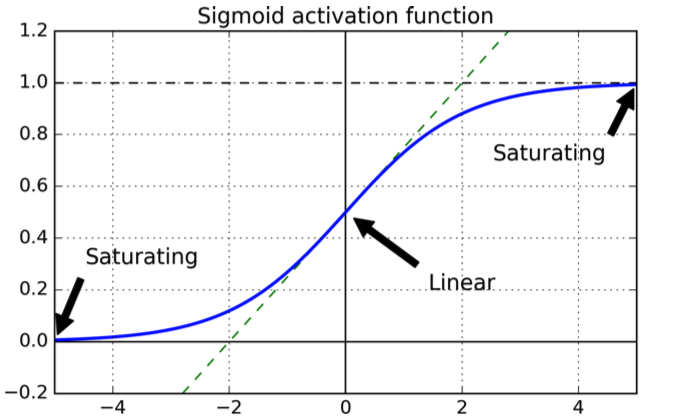
\includegraphics[scale=0.4]{img/sigmoid}
\caption{Sigmoid function.}
\label{sigmoid}
\end{figure}

\subsubsection{Glorot and He initialization}
Glorot and Bengio propose a way to significantly alleviate this prob‐ lem. We need the signal to flow properly in both directions: in the forward direction when making predictions, and in the reverse direction when backpropagating gradi‐ ents. We don’t want the signal to die out, nor do we want it to explode and saturate. For the signal to flow properly, the authors argue that we need the variance of the outputs of each layer to be equal to the variance of its inputs and the gradients to have equal variance before and after flowing through a layer in the reverse direction. It is actually not possible to guarantee both unless the layer has an equal number of inputs and neurons (these numbers are called the fan-in and fan-out of the layer), but they proposed a good compromise that has proven to work very well in practice: the connection weights of each layer must be initialized randomly as

\begin{equation}
\begin{aligned}
\textit{Normal distribution with $0$-mean and variance } \sigma^2 &= \frac{1}{fan_{avg}}\\
\textit{or a Uniform distribution between $[-r, r]$ with } r &= \sqrt{\frac{3}{fan_{avg}}}\\
\textit{with} \textit{ fan}_{avg} &=\frac{\textit{fan}_{in} + \textit{fan}_{out}}{2}
\end{aligned}
\end{equation}
Replacing $\textit{fan}_{avg}$ with $\textit{fan}_{in}$ one gets an initialization strategy proposed by Yann LeCun in 1990s called \ti{LeCun initialization}, which was even recommended in the 1998 book \ti{Neural Networks: Tricks of the Trade by Genevieve Orr and Klaus-Robert Muller (Springer)}. It is equivalent to Glorot initialization when $fan_{in} = fan_{out}$. It took over a decade for researchers to realize just how important this trick really is. Using Glorot initialization can speed up training considerably, and it is one of the tricks that led to the current success of Deep Learning.

Some papers have provided similar strategies for different activation functions. These strategies differ only by the scale of the variance and whether they use $fan_{avg}$ or $fan_{in}$, as shown in \autoref{fig:initial} (for the uniform distribution, just compute $r = 3\sigma^2$). 

\begin{figure}
\centering
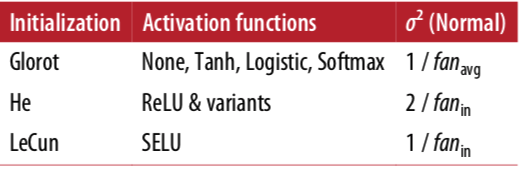
\includegraphics[scale=0.4]{img/initialization}
\caption{Initializations according to the activation functions.}
\label{fig:initial}
\end{figure}
By default, Keras uses Glorot initialization with a uniform distribution. You can change this to He initialization by setting \lstinline+kernel_initializer="he_uniform"+ or \lstinline+kernel_initializer="he_normal"+ when creating a layer.
If you want He initialization with a uniform distribution, but based on $fan_{avg}$ rather
than $fan_{in}$, you can use the \lstinline+VarianceScaling+ initializer like this:
\begin{lstlisting}
he_avg_init = keras.initializers.VarianceScaling(scale=2., mode='fan_avg', distribution='uniform')
keras.layers.Dense(10, activation="sigmoid", kernel_initializer=he_avg_init)
\end{lstlisting}

\subsubsection{Non-saturating activation function: ReLU and SeLU}
The ReLU activation function behaves much better mostly because it does not saturate for positive values (and also because it is quite fast to compute). 
However, it suffers from a problem known as the dying ReLUs: during training, some neurons effectively die, meaning they stop outputting anything other than 0. In some cases, you may find that half of your network’s neurons are dead, especially if you used a large learning rate. A neu‐ ron dies when its weights get tweaked in such a way that the weighted sum of its inputs are negative for all instances in the training set. When this happens, it just keeps outputting 0s, and gradient descent does not affect it anymore since the gradi‐ ent of the ReLU function is 0 when its input is negative.

To solve this problem, you may want to use a variant of the ReLU function, such as the leaky ReLU. This function is defined as
\begin{equation}
\text{LeakyReLU}_\alpha(z) = max(\alpha z, z).
\end{equation}

The hyperparameter $\alpha$ defines how much the function "leaks": it is the slope of the function for $z < 0$, and is typically set to $0.01$. This small slope ensures that leaky ReLUs never die; they can go into a long coma, but they have a chance to eventually wake up. 

Research showed that among several variants of ReLU activation function the leaky variants always outperformed the strict ReLU activation function. In fact, setting $\alpha= 0.2$ (huge leak) seemed to result in better performance than $\alpha = 0.01$ (small leak).
\begin{figure}
\centering
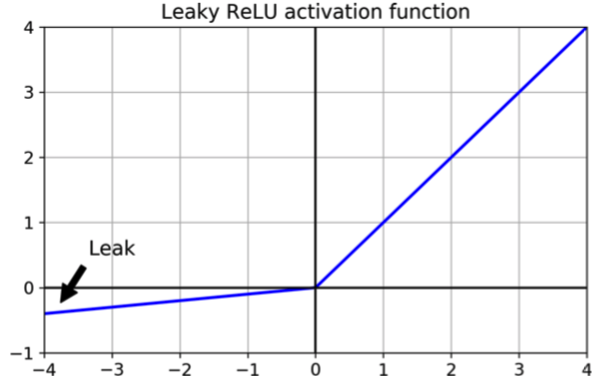
\includegraphics[scale=0.4]{img/lrelu}
\caption{Leaky ReLu activation function.}
\end{figure}
Finally, they also evaluated the parametric leaky ReLU (PReLU), where $\alpha$ is authorized to be learned during training (instead of being a hyperparameter, it becomes a parameter that can be modified by backpropagation like any other parameter). This was reported to strongly outperform ReLU on large image datasets, but on smaller datasets it runs the risk of overfitting the training set. Last but not least, a 2015 paper \footnote{\href{https://homl.info/50}{"Fast and Accurate Deep Network Learning by Exponential Linear Units (ELUs)",  D. Clevert, T. Unterthiner, S. Hochreiter (2015)}} proposed a new activation function called the exponential linear unit (ELU) that outperformed all the ReLU variants in their experiments: training time was reduced and the neural network performed better on the test set. It is represented by:
\begin{equation}
ELU_\alpha(z) = \systeme*{\alpha(e^z - 1) \textit{ if } {z<0} ,z \textit{ if } {z\ge 0}}
\end{equation}
\begin{figure}
\centering
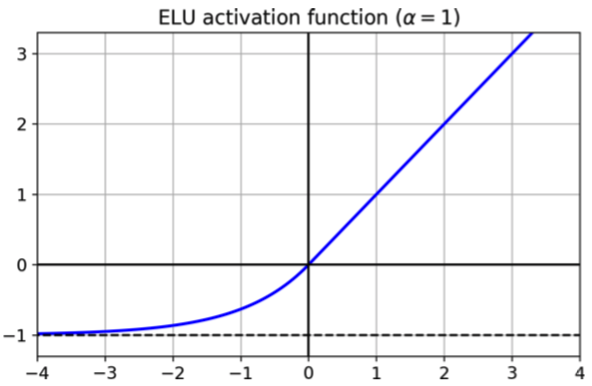
\includegraphics[scale=0.4]{img/ELU}
\caption{ELU activation function.}
\end{figure}
It looks a lot like the ReLU function, with a few major differences:
\begin{itemize}
\item$ First it takes on negative values when z < 0$, which allows the unit to have an average output closer to $0$. This helps alleviate the vanishing gradients problem, as discussed earlier. The hyperparameter $\alpha$ defines the value that the ELU function approaches when $z$ is a large negative number. It is usually set to $1$, but you can tweak it like any other hyperparameter if you want.
\item Second, it has a nonzero gradient for $z < 0$, which avoids the dead neurons problem.
\item Third, if $\alpha$ is equal to $1$ then the function is smooth everywhere, including around $z = 0$, which helps speed up Gradient Descent, since it does not bounce as much left and right of $z = 0$.
\end{itemize}
The main drawback of the ELU activation function is that it is slower to compute than the ReLU and its variants (due to the use of the exponential function), but during training this is compensated by the faster convergence rate. However, at test time an ELU network will be slower than a ReLU network.

Moreover, in a 2017 paper\footnote{\href{https://homl.info/selu}{"Self-Normalizing Neural Networks, " G. Klambauer, T. Unterthiner and A. Mayr (2017).}} by Gunter Klambauer et al., called, the authors showed that if you build a neural network composed exclusively of a stack of dense layers, and if all hidden layers use the SELU activation function (which is just a scaled version of the ELU activation function, as its name suggests), then the network will self-normalize: the output of each layer will tend to preserve mean $0$ and standard deviation $1$ during training, which solves the vanishing/exploding gradients problem. As a result, this activation function often outperforms other activation functions very significantly for such neural nets (especially deep ones). However, there are a few conditions for self-normalization to happen:
\begin{itemize}
\item The input features must be standardized (mean $0$ and standard deviation $1$).
\item Every hidden layer's weights must also be initialized using LeCun normal initialization. In Keras, this means setting \lstinline+kernel_initializer="lecun_norma"+.
\item The network's architecture must be sequential. Unfortunately, if you try to use SELU in non-sequential architectures, such as recurrent networks or networks with skip connections (i.e., connections that skip layers, such as in wide \& deep nets), self-normalization will not be guaranteed, so SELU will not necessarily outperform other activation functions.
\item The paper only guarantees self-normalization if all layers are dense. However, in practice the SELU activation function seems to work great with convolutional neural nets as well.
\end{itemize}

In general $SELU > ELU > \text{leaky }ReLU (and its variants) > ReLU > \tanh > logistic$. If the network's architecture prevents it from self-normalizing, then ELU may perform better than SELU (since SELU is not smooth at $z = 0$). If you care a lot about runtime latency, then you may prefer leaky ReLU. If you don't want to tweak yet another hyperparameter, you may just use the default $\alpha$ values used by Keras (e.g., $0.3$ for the leaky ReLU). If you have spare time and computing power, you can use cross-validation to evaluate other activation functions, in particular RReLU if your network is overfitting, or PReLU if you have a huge training set.
To use the leaky ReLU activation function, you must create a \lstinline+LeakyReLU+ instance like this:
\begin{lstlisting}
leaky_relu = keras.layers.LeakyReLU(alpha=0.2)
layer = keras.layers.Dense(10, activation=leaky_relu, kernel_initializer="he_normal")
\end{lstlisting}
For \lstinline+PReLU+, just replace \lstinline+LeakyRelu(alpha=0.2)+ with \lstinline+PReLU()+.
There is currently no official implementation of RReLU in Keras, but you can fairly easily implement your own. For SELU activation, just set activation="selu" and \lstinline+kernel_initial izer="lecun_normal"+ when creating a layer:
\begin{lstlisting}
layer = keras.layers.Dense(10, activation="selu", kernel_initializer="lecun_normal")
\end{lstlisting}

\subsubsection{Batch normalization}
Although using He initialization along with ELU (or any variant of ReLU) can significantly reduce the vanishing/exploding gradients problems at the beginning of training, it doesn't guarantee that they won't come back during training.

A paper \footnote{"Batch Normalization: Accelerating Deep Network Training by Reducing Internal Covariate Shift", S. Ioffe and C. Szegedy (2015).} proposed a technique called Batch Normalization (BN) to address the vanishing/exploding gradients problems. The technique consists of adding an operation in the model just before or after the activation function of each hidden layer, simply zero-centering and normalizing each input, then scaling and shifting the result using two new parameter vectors per layer: one for scaling, the other for shifting. In other words, this operation lets the model learn the optimal scale and mean of each of the layer's inputs. Typically the normalisation is done before the activation function. In many cases, if you add a BN layer as the very first layer of your neural network, you do not need to standardize your training set (e.g., using a \lstinline+StandardScaler+): the BN layer will do it for you (well, approximately, since it only looks at one batch at a time, and it can also rescale and shift each input feature).

In order to zero-centre and normalize the inputs, the algorithm needs to estimate each input's mean and standard deviation. It does so by evaluating the mean and standard deviation of each input over the current mini-batch (hence the name "Batch Normalization"). The whole operation is summarized in \autoref{eq:BatchNormalisation}

\begin{equation}
\begin{aligned}
\mathbf{\mu_B} &= \frac{1}{m_B} \sum_{i=1}^{m_B} \x^{(i)} \\
\mathbf{\sigma}_B^2 &= \frac{1}{m_B} \sum_{i=1}^{m_B} \br{\x^{(i)} - \mathbf{\mu}_B}^2\\
\hat{\mathbf{x}}^{(i)} &= \frac{\x^{(i)} - \mathbf{\mu}_B}{\sqrt{\mathbf{\sigma}_B^2 +\epsilon}}\\
\mathbf{z}^{(i)} &= \mathbf{\gamma} \otimes \hat{\mathbf{x}}^{(i)} + \mathbf{\beta}
\end{aligned}
\label{eq:BatchNormalisation}
\end{equation}
where $\mathbf{\mu}_B$ is the vector of input means and $\sigma_B$ is the vector of input standard deviation both evaluated over the whole mini-batch $B$. $m_B$ is the number of instances in the mini-batch, $\hat{\mathbf{x}}^{(i)}$ is the vector of zero-centred and normalized inputs for instance $i$.

It is not always desirable to have hidden units with $0$ mean and variace $1$. For example consider the values are the input to a sigmoid function: it might be better to have a higher values in order to exploit the non-linearities of the function. So we introduce the learning parameters $\gamma$ and $\beta$ to get a different distribution. $\gamma$ is the output scale parameter vector layer (it contains one scale parameter vector for the layer), $\otimes$ represents element-wise multiplication (each element is multiplied by its corresponding output scale parameter), $\beta$ is the output shift parameter vector for the layer. Each input is offset by its corresponding shift parameter, $\epsilon$ is a small positive quantity to avoid division by $0$ and it is called \tb{smoothing term}, $\mathbf{z}^{(i)}$ is the output of the BN operation, a rescaled and shifted version of the inputs.

Note that the learning parameter $b$ gets cancelled out by BN normilise the batch to have $0$ mean and standard deviation $1$ and then rescale by $\beta$ and $\gamma$. So the parameter $b$ can be completely ignore or set permanently to $0$.

\tb{Batch normalisation can be used together with other optimisation algorithm such as Momentum, RMSProp, Adam, etc.}.

\paragraph{\tb{Why does Batch normalisation work?}} Consider a NN for cat detection task trained only on black cats. When applied to images with coloured cats, the classifier might not be doing well due to the different distribution of data that the NN has never seen. The idea of the data distribution change goes behind the name of \tb{Covariate Shift}. In this case the algorithm needs retraining. From the perspective of a hidden layer, its input activation values changes due to the changes in the learning parameter of the earlier layers and so suffering of the problem of covariance shift. BN reduce the amount of the shift by forcing to have the same mean and variance $\beta$ and $\gamma$. \tb{It limits the amount to which updating the parameters in the earlier layers can affect the distribution of values seen by the deeper hidden layers}. It causes the input values of the later layers to be more stable allowing each layer to learn a little more independently from the others.

One may need to make predictions for individual instances rather than for batches of instances: in this case, we will have no way to compute each input's mean and standard deviation. Moreover, even if we do have a batch of instances, it may be too small, or the instances may not be independent and identically distributed (IID), so computing statistics over the batch instances would be unreliable (during training, the batches should not be too small, if possible more than $30$ instances, and all instances should be IID). One solution could be to wait until the end of training, then run the whole training set through the neural network, and compute the mean and standard deviation of each input of the BN layer. These "final" input means and standard deviations can then be used instead of the batch input means and standard deviations when making predictions. However, it is often preferred to estimate these final statistics during training using a exponentially weighted average of the layer's input means and standard deviations. To sum up, four parameter vectors are learned in each batch-normalized layer: $\gamma$ (the output scale vector) and $\beta$ (the output offset vector) are learned through regular backpropagation, and $\mu$ (the final input mean vector), and $\sigma$ (the final input standard deviation vector) are estimated using an exponential moving average. Note that $\mu$ and $\sigma$ are estimated during training, but they are not used at all during training, only after training.

The vanishing gradients problem was strongly reduced, to the point that they could use saturating activation functions such as the $\tanh$ and even the logistic activation function. The networks were also much less sensitive to the weight initialization. They were able to use much larger learning rates, significantly speeding up the learning process.
 
You may find that training is rather slow, because each epoch takes much more time when you use batch normalization. However, this is usually counterbalanced by the fact that convergence is much faster with BN, so it will take fewer epochs significantlyto reach the same performance. All in all, wall time will usually be smaller (this is the time measured by the clock on your wall). 
 
\paragraph{\tb{Drawbacks}} Batch Normalization does, however, add some complexity to the model (although it can remove the need for normalizing the input data, as we discussed earlier). Moreover, there is a runtime penalty: the neural network makes slower predictions due to the extra computations required at each layer. So if you need predictions to be lightning-fast, you may want to check how well plain ELU $+$ He initialization perform before playing with Batch Normalization. 

\paragraph{\tb{BN as regularisation}} Computing mean and variance for each mini batch means introducing some noise that result in a slight regularisation effect.

\subsubsection{Implementing BN in keras}
Just add a BatchNormalization layer before or after each hidden layer's activation function, and optionally add a BN layer as well as the first layer in your model. For example, this model applies BN after every hidden layer and as the first layer in the model (after flattening the input images):
\begin{lstlisting}
model = keras.models.Sequential([
        keras.layers.Flatten(input_shape=[28, 28]),
        keras.layers.BatchNormalization(),
        keras.layers.Dense(300, activation="elu", kernel_initializer="he_normal"),
        keras.layers.BatchNormalization(),
        keras.layers.Dense(100, activation="elu", kernel_initializer="he_normal"),
        keras.layers.BatchNormalization(),
        keras.layers.Dense(10, activation="softmax")
])
\end{lstlisting}
Each BN layer adds 4 parameters per input (for example, the first BN layer adds $3136$ parameters, which is 4 times $784$). $\mu$ and $\sigma$ are the moving averages, they are not affected by backpropagation, so Keras calls them "Non-trainable", while $\gamma, \beta$ are.

Now when you create a BN layer in Keras, it also creates two operations that will be called by Keras at each iteration during training. These operations will update the moving averages. Since we are using the TensorFlow backend, these operations are TensorFlow operations.

The authors of the BN paper argued in favour of adding the BN layers before the activation functions, rather than after (as we just did). There is some debate about this, as it seems to depend on the task. So that's one more thing one can experiment with to see which option works best on your dataset. To add the BN layers before the activation functions, we must remove the activation function from the hidden layers, and add them as separate layers after the BN layers. Moreover, since a Batch Normalization layer includes one offset parameter per input, you can remove the bias term from the previous layer (just pass \cd+use_bias=False+ when creating it):
\begin{lstlisting}
model = keras.models.Sequential([
        keras.layers.Flatten(input_shape=[28, 28]),
        keras.layers.BatchNormalization(),
        keras.layers.Dense(300, kernel_initializer="he_normal", use_bias=False),
        keras.layers.BatchNormalization(),
        keras.layers.Activation("elu"),
        keras.layers.Dense(100, kernel_initializer="he_normal", use_bias=False),
        keras.layers.Activation("elu"),
        keras.layers.BatchNormalization(),
        keras.layers.Dense(10, activation="softmax")
])
\end{lstlisting}
The \cd+BatchNormalization+ class has quite a few hyperparameters you can tweak. The defaults will usually be fine, but you may occasionally need to tweak the \cd+momentum+. This hyperparameter is used when updating the exponential moving averages: given a new value $\mathbf{v}$ (i.e., a new vector of input means or standard deviations computed over the current batch), the running average $\hat{\mathbf{v}}$ is updated using the following equation:
\begin{equation}
\hat{\mathbf{v}} \leftarrow \hat{\mathbf{v}} \times momentum + \mathbf{v} \br{1-momentum}
\end{equation}
A good momentum value is typically close to $1$, where the larger the dataset or the smaller the mini-batch, the closer to $1$.

Another important hyperparameter is \cd+axis+: it determines which axis should be normalized. It defaults to $=1$, meaning that by default it will normalize the last axis (using the means and standard deviations computed across the other axes). For example, when the input batch is 2D (i.e., the batch shape is \cd+[batch size, features]+), this means that each input feature will be normalized based on the mean and standard deviation computed across all the instances in the batch. For example, the first BN layer in the previous code example will independently normalize (and rescale and shift) each of the 784 input features. However, if we move the first BN layer before the \cd+Flatten+ layer, then the input batches will be 3D, with shape \cd+[batch size, height, width]+, therefore the BN layer will compute 28 means and 28 standard deviations. There will also be just 28 scale parameters and 28 shift parameters. If instead you still want to treat each of the 784 pixels independently, then you should set \cd+axis=[1, 2]+.

Batch Normalization has become one of the most used layers in deep neural networks, to the point that it is often omitted in the diagrams, as it is assumed that BN is added after every layer. However, a very recent paper\footnote{"Fixup Initialization: Residual Learning Without Normalization", Hongyi Zhang, Yann N. Dauphin, Tengyu Ma (2019).} may well change this: the authors show that by using a novel fixed-update (fixup) weight initialization technique, they manage to train a very deep neural network (10,000 layers) without BN, achieving state-of-the-art performance on complex image classification tasks.

\subsubsection{Gradient clipping}
Another popular technique to lessen the exploding gradients problem is to simply clip the gradients during backpropagation so that they never exceed some threshold. This is called Gradient Clipping\footnote{\href{https://homl.info/52}{"On the difficulty of training recurrent neural networks", R. Pascanu et al. (2013).}}. This technique is most often used in recurrent neural networks, as Batch Normalization is tricky to use in RNNs. For other types of networks, BN is usually sufficient.

In Keras, implementing Gradient Clipping is just a matter of setting the \cd+clipvalue+ or \cd+clipnorm+ argument when creating an optimizer. For example:
\begin{lstlisting}
optimizer = keras.optimizers.SGD(clipvalue=1.0)
model.compile(loss="mse", optimizer=optimizer)
\end{lstlisting}
This will clip every component of the gradient vector to a value between $-1.0$ and $1.0$. This means that all the partial derivatives of the loss (with regards to each and every trainable parameter) will be clipped between $-1.0$ and $1.0$. The threshold is a hyperparameter you can tune. Note that it may change the orientation of the gradient vector: for example, if the original gradient vector is $[0.9, 100.0]$, it points mostly in the direction of the second axis, but once you clip it by value, you get $[0.9, 1.0]$, which points roughly in the diagonal between the two axes. In practice however, this approach works well. If you want to ensure that Gradient Clipping does not change the direction of the gradient vector, you should clip by norm by setting \cd+clipnorm+ instead of \cd+clipvalue+. This will clip the whole gradient if its $L2$ norm is greater than the threshold you picked. For example, if you set \cd+clipnorm=1.0+, then the vector $[0.9, 100.0]$ will be clipped to $[0.00899964, 0.9999595]$, preserving its orientation, but almost eliminating the first component. If you observe that the gradients explode during training (you can track the size of the gradients using TensorBoard), you may want to try both clipping by value and clipping by norm, with different threshold, and see which option performs best on the validation set.

\subsection{Reusing Pretrained Layers}
It is generally not a good idea to train a very large DNN from scratch: instead, you should always try to find an existing neural network that accomplishes a similar task to the one you are trying to tackle, then just reuse the lower layers of this network: this is called \tb{transfer learning}. If the input pictures of your new task don't have the same size as the ones used in the original task, you will usually have to add a preprocessing step to resize them to the size expected by the original model. More generally, transfer learning will work best when the inputs have similar low-level features.

The output layer of the original model should usually be replaced since it is most likely not useful at all for the new task, and it may not even have the right number of outputs for the new task. Similarly, the upper hidden layers of the original model are less likely to be as useful as the lower layers, since the high-level features that are most useful for the new task may differ significantly from the ones that were most useful for the original task. You want to find the right number of layers to reuse.

Try freezing all the reused layers first (i.e., make their weights non-trainable, so gradient descent won't modify them), then train your model and see how it performs. Then try unfreezing one or two of the top hidden layers to let backpropagation tweak them and see if performance improves. The more training data you have, the more layers you can unfreeze. It is also useful to reduce the learning rate when you unfreeze reused layers: this will avoid wrecking their fine-tuned weights. 
Similarly, the upper hidden layers of the original model are less likely to be as useful as the lower layers, since the high-level features that are most useful for the new task may differ significantly from the ones that were most useful for the original task. You want to find the right number of layers to reuse.
The more similar the tasks are, the more layers you want to reuse (starting with the lower layers). For very similar tasks, you can try keeping all the hidden layers and just replace the output layer.
Try freezing all the reused layers first (i.e., make their weights non-trainable, so gradi‐ ent descent won’t modify them), then train your model and see how it performs. Then try unfreezing one or two of the top hidden layers to let backpropagation tweak them and see if performance improves. The more training data you have, the more layers you can unfreeze. It is also useful to reduce the learning rate when you unfreeze reused layers: this will avoid wrecking their fine-tuned weights.
If you still cannot get good performance, and you have little training data, try drop‐ ping the top hidden layer(s) and freeze all remaining hidden layers again. You can iterate until you find the right number of layers to reuse. If you have plenty of training data, you may try replacing the top hidden layers instead of dropping them, and even add more hidden layers.

\subsubsection{Transfer learning with keras}
Suppose from a multinomial classifier one wants a new binary classifier whose classes were among the multinomial classifier. Let's reuse all layers except for the output layer:
\begin{lstlisting}
model_A = keras.models.load_model("my_model_A.h5")
model_B_on_A = keras.models.Sequential(model_A.layers[:-1])
model_B_on_A.add(keras.layers.Dense(1, activation="sigmoid"))
\end{lstlisting}
Note that \cd+model_A+ and \cd+model_B_on_A+ now share some layers. When you train \cd+model_B_on_A+, it will also affect \cd+model_A+. If you want to avoid that, you need to clone \cd+model_A+ before you reuse its layers. To do this, you must clone model $A$'s architecture, then copy its weights (since \cd+clone_model()+ does not clone the weights):
\begin{lstlisting}
model_A_clone = keras.models.clone_model(model_A)
model_A_clone.set_weights(model_A.get_weights())
\end{lstlisting}
Now we could just train \cd+model_B_on_A+ for task B, but since the new output layer was initialized randomly, it will make large errors, at least during the first few epochs, so there will be large error gradients that may wreck the reused weights. To avoid this, one approach is to freeze the reused layers during the first few epochs, giving the new layer some time to learn reasonable weights. To do this, simply set every layer's trainable attribute to \d+False+ and compile the model (\tb{one must always compile your model after one freezes or unfreezes layers.}
\begin{lstlisting}
for layer in model_B_on_A.layers[:-1]:
    layer.trainable = False
model_B_on_A.compile(loss="binary_crossentropy", optimizer="sgd", metrics=["accuracy"])
\end{lstlisting}
Next, we can train the model for a few epochs, then unfreeze the reused layers (which requires compiling the model again) and continue training to fine-tune the reused layers. After unfreezing the reused layers, it is usually a good idea to reduce the learning rate, once again to avoid damaging the reused weights:
\begin{lstlisting}
 history = model_B_on_A.fit(X_train_B, y_train_B, epochs=4, validation_data=(X_valid_B, y_valid_B))
for layer in model_B_on_A.layers[:-1]: layer.trainable = True
    optimizer = keras.optimizers.SGD(lr=1e-4) # the default lr is 1e-3 model_B_on_A.compile(loss="binary_crossentropy", optimizer=optimizer, metrics=["accuracy"])
history = model_B_on_A.fit(X_train_B, y_train_B, epochs=16, validation_data=(X_valid_B, y_valid_B))
\end{lstlisting}
\tb{Actually using this method is cheating. If one tries to change the classes or the random seed, the improvement generally drops, or even vanishes or reverses. It turns out that transfer learning does not work very well with small dense networks: it works best with deep convolutional neural networks}.

\subsubsection{Unsupervised pretraining}
Suppose you cannot find a model trained on a similar task for a complex task for which you don't have enough data. First, you should of course try to gather more labeled training data, but if this is too hard or too expensive, you may still be able to perform \tb{unsupervised pretraining}.  It is often rather cheap to gather unlabeled training examples, but quite expensive to label them. If you can gather plenty of unlabeled training data, you can try to train the layers one by one, starting with the lowest layer and then going up, using an unsupervised feature detector algorithm such as Restricted Boltzmann Machines or autoencoders. Each layer is trained on the output of the previously trained layers (all layers except the one being trained are frozen). Once all layers have been trained this way, you can add the output layer for your task, and fine-tune the final network using supervised learning. At this point, you can unfreeze all the pretrained layers, or just some of the upper ones. This is a rather long and tedious process, but it often works well.

\subsubsection{Pretraining on an auxiliary task}
If you do not have much labeled training data, one last option is to train a first neural network on an auxiliary task for which you can easily obtain or generate labeled training data, then reuse the lower layers of that network for your actual task. The first neural network's lower layers will learn feature detectors that will likely be reusable by the second neural network.

For example, if you want to build a system to recognize faces, you may only have a few pictures of each individual - clearly not enough to train a good classifier. Gatheing hundreds of pictures of each person would not be practical. However, you could gather a lot of pictures of random people on the web and train a first neural network to detect whether or not two different pictures feature the same person. Such a network would learn good feature detectors for faces, so reusing its lower layers would allow you to train a good face classifier using little training data.

\subsubsection{Speed up training with transfer learning}
Since the early layers are fixed, one can think that the input layer is now the output of the last frozen layer: in fact, its output, given an image, does not change because all parameters of the previous layers have been fixed and are known. To speed up the training of the new layers, one can pre-compute the output of the frozen layer and save it to disk. This input is then used to train the new layers as if it were a shallow network. Since the inputs are always the same and the weights and biases of early layers are constant, this operation saves time because many repeated operations are avoided.

\subsection{Faster optimisation}
Another huge speed boost comes from using a faster optimizer than the regular Gradient Descent optimizer. Other optimizers are:
\begin{itemize}
\item Momentum optimisation
\item Nesterov Accelerated Gradient
\item AdaGrad
\item RMSProp
\item Adam and Nadam optimisation
\end{itemize}

\subsubsection{Exponentially weighted averages}
\label{subsubsec:ExpWeightedAvg}
To understand optimisation algorithms to the full, one must get the idea behind them. Some optimisations are based on the exponentially weighted averages.

Given a series $\theta_i, i=1,\cdots, n$, the exponential weighted average consists of setting an initial vaue $v_0$, typically initialised to $0$, and to compute the other elements of the output series as:
\begin{equation}
\begin{aligned}
v_0 &= 0\\
v_i &= \beta v_{i-1}+(1-\beta) \theta_i 
\end{aligned}
\end{equation}
This can be re-written as:
\begin{equation}
v_i = (1-\beta) \theta_i +  (1-\beta) \beta \theta_{i-1} + (1-\beta) \beta^2 \theta_{i-2} + (1-\beta) \beta^3 \theta_{i-3} + \cdots  
\end{equation}
which is exponentially decaying. All the coefficients add up to very close to one up to a detail called bias correction.

This filtering smooths the samples by taking into account all the previous values of the sries with decreasing emphasis. Particularly, $v_i$ is said to be the average over the previous $\approx \frac{1}{1-\beta}$ number of samples. So, increasing $\beta$ results in higher smoothing, however due to the larger averaging window, the delay is bigger and the resuling curve will be right-shifted \autoref{img:expAvg}	. In fact, setting for example $\beta=0.9$, $0.9^{10}\approx 0.35 \approx \frac{1}{e}$. Naming $1-\beta=\epsilon=0.1$, $(1-\epsilon)^\epsilon=\frac{1}{e}$. It takes $10$ samples for the initial value to decay of $\frac{1}{e}$, about a third. On the contrast, if $\beta=0.98$, $0.98^{50}\approx \frac{1}{e}$. This is of course a rule of thumb of how to think about it, not a formal mathematical statement.	

\begin{figure}
\centering
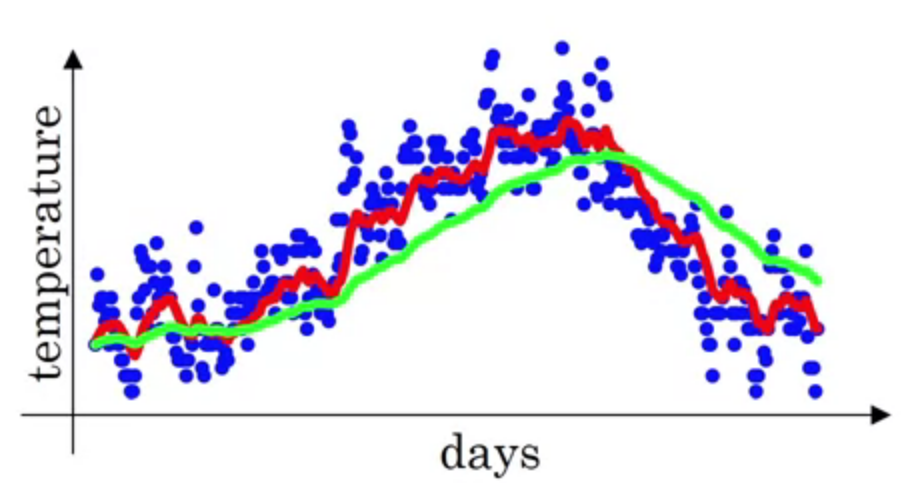
\includegraphics[scale=0.3]{img/expAvg}
\caption{Exampe of exponentially averaging with $\beta=0.9$ in red and $\beta=0.98$ in green.}
\label{img:expAg}
\end{figure}

\subsubsection{Bias correction of exponentially weighted aerages}
If we initialise $v_0=0$ then $v_1= (1-\beta) \theta_1$, so the first point can be out of scale, particularly too small, compared to the values of $\theta$, so the first estimates can be wrong. Instead of taking $v_i$, the solution is to take $\frac{v_i}{1-\beta^i}$, so we are dividing by a quantity smaller than $1$.

\subsubsection{Momentum optimisation}
\label{subsubsec:momentum}
Gradient Descent simply updates the weights by directly subtracting the gradient of the cost function  with regards to the weights multiplied by the learning rate: it does not care about what the earlier gradients were. If the local gradient is tiny, it goes very slowly. Momentum optimization consists of using exponentially weighted averages in order to take into account previous gradients. \autoref{img:gradientSteps} shows for an elliptic cost funtion the oscillations of the gradient algorithm that slow down the algorithm and that prevents from using a larger learning rate which would cause overshooting and possibly diverging. In other words, on the vertical axis one wants the learning to be slower to avoid the oscillations and faster learning on the horizontal axis.

The exponentially weighted average sums the previous components of the gradient: the vertical components have opposite directions so they are getting subtracted and the final vertical component is strongly reduced to a quantity close to $0$. On the horizontal axis, the derivatives are all pointing to the same direction so the average on the horizontal direction will still be pretty big. So once one has computed the derivatives, instead of using them directly, use the exponentially weighted average to update the weights. This allows the algorithm to take a more straightforward path. In practice, \tb{bias correction is seldom used} but it does not hurt.

The upgrade equations become:
\begin{equation}
\begin{aligned}
v &\leftarrow \beta v - (1-\beta) \nabla_\theta J(\theta)\\
\theta &\leftarrow \theta - \eta \theta
\end{aligned}
\end{equation}
More commonly the equations are written omitting $(1-\beta)$:
\begin{equation}
\begin{aligned}
m &\leftarrow \beta m - \eta \nabla_\theta J(\theta)\\
\theta &\leftarrow \theta + m
\end{aligned}
\end{equation}
This is pretty much identical to the first pair of equation, the only difference is that you need to scale learning rate by $1-\beta$ factor, and possibly retune the learning rate.

\begin{figure}
\centering
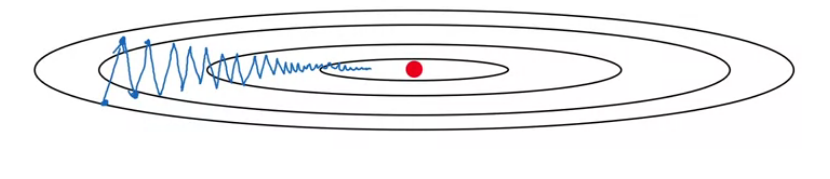
\includegraphics[scale=0.45]{img/momentum}
\caption{Example of gradient steps.}
\label{img:gradientSteps}
\end{figure}

Often the analogy of a ball rolling down a surface is used
\footnote{\href{https://homl.info/54}{"Some methods of speeding up the convergence of iteration methods", B. Polyak (1964).}}: a rolling ball on a gentle slope will start out slowly but will pick up a momentum until it reaches a terminal velocity due to some friction or air resistance. The friction is represented by $\beta$ (smaller than $1$) which prevents the mometum from becoming too large: $0$ (high friction) and $1$ (no friction). A typical $\beta$ value is $0.9$.

One can easily verify that if the gradient remains constant, the terminal velocity (i.e., the maximum size of the weight updates) is equal to that gradient multiplied by the learning rate $\eta$ multiplied by $\frac{1}{1-\beta}$ (ignoring the sign). For example, if $\beta = 0.9$, then the terminal velocity is equal to $10$ times the gradient times the learning rate, so Momentum optimization ends up going $10$ times faster than Gradient Descent! This allows Momentum optimization to escape from plateaus much faster than Gradient Descent.

In deep neural networks that don't use Batch Normalization, the upper layers will often end up having inputs with very different scales, so using Momentum optimization helps a lot. It can also help roll past local optima. Due to the momentum, the optimizer may overshoot a bit, then come back, overshoot again, and oscillate like this many times before stabilizing at the minimum. This is one of the reasons why it is good to have a bit of friction in the system: it gets rid of these oscillations and thus speeds up convergence. 

Implementing Momentum optimization in Keras is a no-brainer: just use the SGD optimizer and set its \lstinline+momentum+ hyperparameter which represent the $\beta$ parameter in the previous equations:
\begin{lstlisting}
optimizer = keras.optimizers.SGD(lr=0.001, momentum=0.9)
\end{lstlisting}
The one drawback of Momentum optimization is that it adds yet another hyperpara‐ meter to tune. However, the momentum value of $0.9$ usually works well in practice and almost always goes faster than regular Gradient Descent and can also be applied with the same improvement to mini-batch gradient descent.

\subsubsection{Nesterov accelerated gradient}\footnote{\href{https://homl.info/55}{"A Method for Unconstrained Convex Minimization Problem with the Rate of Convergence $O(1/k^2)$", Yurii Nesterov (1983).}}

The idea of Nesterov Momentum optimization, or Nesterov Accelerated Gradient (NAG), is to measure the gradient of the cost function not at the local position but slightly ahead in the direction of the momentum. The only difference from vanilla Momentum optimization is that the gradient is measured at $\theta + \beta m$:
\begin{equation}
\begin{aligned}
m &\leftarrow \beta m - \eta \nabla_\theta J(\theta+\beta m)\\
\theta &\leftarrow \theta + m
\end{aligned}
\end{equation}
This small tweak works because in general the momentum vector will be pointing in the right direction (i.e., toward the optimum), so it will be slightly more accurate to use the gradient measured a bit farther in that direction rather than using the gradient at the original position. Suppose $\nabla_1$ represents represents the gradient of the cost function measured at the starting point $\theta$, and $\nabla_2$ gradient at the point located at $\theta + \beta m$. This small tweak works because in general the momentum vector will be pointing in the right direction (i.e., toward the optimum), so it will be slightly more accurate to use the gradient measured a bit farther in that direction rather than using the gradient at the original position. After a while, these small improvements add up and NAG ends up being significantly faster than regular Momentum optimization. Moreover, note that when the momentum pushes the weights across a valley, $\nabla_1$ continues to push further across the valley, while $\nabla_2$ pushes back toward the bottom of the valley. NAG will almost always speed up training compared to regular Momentum optimisation. To use it, simply set \cd+nesterov=True+ when creating the SGD optimizer:
\begin{lstlisting}
optimizer = keras.optimizers.SGD(lr=0.001, momentum=0.9, nesterov=True)
\end{lstlisting}
\begin{figure}
\centering
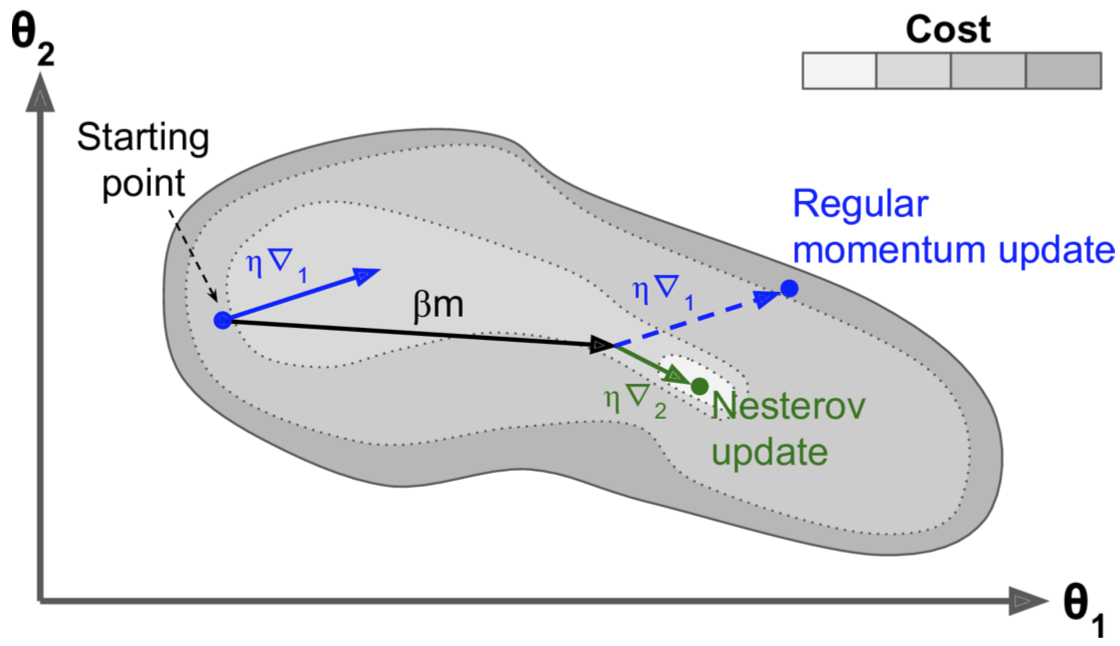
\includegraphics[scale=0.5]{img/nesterov}
\caption{Nesterov momentum.}
\end{figure}
\subsubsection{AdaGrad}
Consider the elongated bowl problem again: Gradient Descent starts by quickly going down the steepest slope, then slowly goes down the bottom of the valley. It would be nice if the algorithm could detect this early on and correct its direction to point a bit more toward the global optimum. The \tb{Adagrad algorithm}\footnote{\href{https://homl.info/56}{"Adaptive Subgradient Methods for Online Learning and Stochastic Optimization", J. Duchi et al. (2011).}} achieves this by scaling down the gradient vector along the steepest dimensions:
\begin{equation}
\begin{aligned}
a &\leftarrow s + \nabla_\theta J(\theta) \otimes \nabla_\theta J(\theta)\\
\theta &\leftarrow \theta - \eta  \nabla_\theta J(\theta) \oslash \sqrt{s+\epsilon}
\end{aligned}
\end{equation}
The first step accumulates the square of the gradients into the vector $s$. If the cost function is steep along the i-th dimension, then $s_i$ will get larger and larger at each iteration. The second step is almost identical to Gradient Descent, but with one big difference: the gradient vector is scaled down by a factor of $\sqrt{s+\epsilon}$ where the $\oslash$ symbol represents the element-wise division and $\epsilon$ is to avoid division by $0$.

In short, this algorithm decays the learning rate, but it does so faster for steep dimensions than for dimensions with gentler slopes. This is called an \tb{adaptive learning rate}. One additional benefit is that it requires much less tuning of the learning rate hyperparameter $\eta$. Looking at \autoref{fig:adagrad}, it is like with adagrad, the path to reach the minimum is shorter.

\begin{figure}
\centering
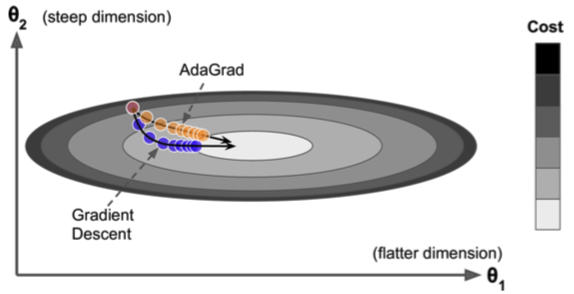
\includegraphics[scale=0.5]{img/adagrad}
\caption{AdaGrad optimisation.}
\label{fig:adagrad}
\end{figure}
AdaGrad often performs well for simple quadratic problems, but unfortunately it often stops too early when training neural networks. The learning rate gets scaled down so much that the algorithm ends up stopping entirely before reaching the global optimum. So even though Keras has an \cd+Adagrad+ optimizer, you should not use it to train deep neural networks (it may be efficient for simpler tasks such as Linear Regression, though). 

\subsubsection{RMSProp}
\label{subsec:RMSprop}
The RMSProp (Root Mean Square prop) algorithm\footnote{This algorithm was created by Geoffrey Hinton and Tijmen Tieleman in 2012, and presented by Geoffrey Hinton in his Coursera class on neural networks (\href{slides}{https://homl.info/57}; \href{video}{https://homl.info/58}). Amusingly, since the authors did not write a paper to describe it, researchers often cite "slide 29 in lecture 6" in their papers.} fixes Adagrad non-convergence by accumulating only the gradients from the most recent iterations (as opposed to all the gradients since the beginning of training). It does so by using exponential decay in the first step as done in the momentum algorithm (\autoref{subsubsec:momentum}), but instead of averaging over the derivatives, it aerage over the (element-wise) squared derivatives and the gradient in the update equation is divided by the square root of the average:
\begin{equation}
\begin{aligned}
s &\leftarrow \beta s + (1-\beta) \nabla_\theta J(\theta) \otimes \nabla_\theta J(\theta)\\
\theta &\leftarrow \theta - \eta \nabla_\theta J(\theta) \oslash \sqrt{s+\epsilon}
\end{aligned}
\end{equation}
The decay rate $\beta$ is typically set to $0.9$. It is once again a new hyperparameter, but this default value often works well, so you may not need to tune it at all.

Keras has an \cd+RMSProp+ optimizer:
\begin{equation}
\begin{aligned}
optimizer = keras.optimizers.RMSprop(lr=0.001, rho=0.9)
\end{aligned}
\end{equation}
The goal of this algorithm is to dump the oscillations as in the momentum algorithm. In fact $s$ is the average of the derivatives: it will have high absolute values in the directions of oscillations (since an oscillation means a rapid change) and small values in the "stable" directions. Since the root sqaure is used as denominator in the update equation, it dumps the terms with high oscillations (high valus of $s$) and increase the terms with oscillations close to $0$. Except on very simple problems, this optimizer almost always performs much better than AdaGrad. In fact, it was the preferred optimization algorithm of many researchers until Adam optimization came around.


\subsubsection{Adam and Nadam Optimisation}
\label{subsec:ADAM}
\tb{Adam}\footnote{\href{https://homl.info/59}{"Adam: A Method for Stochastic Optimization", D. Kingma, J. Ba (2015).}}, which stands for \tb{Adaptive Moment estimation}, combines the ideas of Momentum optimization and RMSProp: just like Momentum optimization it keeps track of an exponentially decaying average of past gradients, and just like RMSProp it keeps track of an exponentially decaying average of past squared gradients. Adam does use bias correction.

\begin{equation}
\begin{aligned}
m_0 &\leftarrow 0\\
s_0 &\leftarrow 0\\
m &\leftarrow \beta_1 m + \br{1-\beta_1} \nabla_\theta J(\theta)\\
s &\leftarrow \beta_2 s + (1-\beta_2) \nabla_\theta J(\theta) \otimes \nabla_\theta J(\theta)\\
\hat{m} &\leftarrow\frac{m}{1-\beta_1^t}\\
\hat{s} &\leftarrow\frac{s}{1-\beta_2^t}\\
\theta &\leftarrow \theta - \eta \hat{m} \oslash (\sqrt{\hat{s}}+\epsilon)
\end{aligned}
\label{eq:Adam}
\end{equation}
where $t$ is the iteration number starting at $1$. $\beta_1$ is typically $0.9$ and $\beta_2$ $0.999$. $\epsilon$ does not really matter but the author of the paper recommended $10^{-8}$.

\begin{lstlisting}
optimizer = keras.optimizers.Adam(lr=0.001, beta_1=0.9, beta_2=0.999)
\end{lstlisting}
Since Adam is an adaptive learning rate algorithm (like AdaGrad and RMSProp), it requires less tuning of the learning rate hyperparameter $\eta$. You can often use the default value $\eta = 0.001$, making Adam even easier to use than Gradient Descent.

Two variants of Adam exist:
\begin{itemize}
\item \tb{Adamax}, introduced in the same paper of Adam, \autoref{eq:Adam}, Adam accumulates the squares of the gradients in $s$ (with a greater weight for more recent weights). If we ignore $\epsilon$ and the bias corrections, Adam just scales down the parameter updates by the square root of $s$. In short, Adam scales down the parameter updates by the $L2$ norm of the time-decayed gradients (recall that the $L2$ norm is the square root of the sum of squares). Adamax just replaces the $L_2$ norm with the $L_\infty$ norm (a fancy way of saying the maximum). Specifically, the RMSProp step is replaced by:
\begin{equation}
s \leftarrow max\br{\beta_2 s, \nabla_\theta J(\theta)},
\end{equation}
and scales the gradient updates by a factor of $s$, which is just the max of the time-decayed gradients. This can make Adamax more stable than Adam, but this really depends on the dataset, and in general Adam actually performs better.
\item \tb{Nadam optimisation}\footnote{\href{https://homl.info/nadam}{"Incorporating Nesterov Momentum into Adam", Timothy Dozat (2015).}} is simply Adam optimization plus the Nesterov trick, so it will often converge slightly faster than Adam. 
\end{itemize}

Adaptive optimization methods (including RMSProp, Adam and Nadam optimization) are often great, converging fast to a good solution. However, a 2017 paper \footnote{\href{https://homl.info/60}{"The Marginal Value of Adaptive Gradient Methods in Machine Learning", A. C. Wilson et al. (2017).}} showed that they can lead to solutions that generalize poorly on some datasets. So when you are disappointed by your model's performance, try using plain Nesterov Accelerated Gradient instead: your dataset may just be allergic to adaptive gradients.

Algorithms based on second derivatives become too hard to apply.

\paragraph{\tb{Sparse model}} All the optimization algorithms just presented produce dense models, meaning that most parameters will be nonzero. If you need a blazingly fast model at runtime, or if you need it to take up less memory, you may prefer to end up with a sparse model instead. One trivial way to achieve this is to train the model as usual, then get rid of the tiny weights (set them to 0). However, this will typically not lead to a very sparse model, and it may degrade the model's performance. A better option is to apply strong $L_1$ regularization during training, as it pushes the optimizer to zero out as many weights as it can. However, in some cases these techniques may remain insufficient. One last option is to apply Dual Averaging, often called Follow The Regularized Leader (FTRL)\footnote{\href{However, in some cases these techniques may remain insufficient. One last option is to apply Dual Averaging, often called Follow The Regularized Leader (FTRL)}{"Primal-Dual Subgradient Methods for Convex Problems"s, Yurii Nesterov (2005).}}

\subsection{Learning rate scheduling}
As already stated one approach is to start with a large learning rate, and divide it by 3 until the training algorithm stops diverging. A better approach is a variable learning rate. Here are different learning scheduled
\begin{itemize}
\item \tb{Power scheduling} Set the learning rate to a function of the iteration number $t$:
\begin{equation}
\eta(t) = \frac{\eta_0}{\br{1+\frac{t}{k}}^c}
\end{equation}
where $c$ is typically $1$. The learning rate drops at each step. After $s$ steps it is down to $\eta_0 / 2$. After $s$ more steps, it is down to $\eta_0 / 3$. Then down to $\eta_0 / 4$, then $\eta_0 / 5$ and so on. This schedule first drops quickly, then more and more slowly. Of course, this requires tuning $\eta_0$, $s$ (and possibly $c$).
\item \tb{Exponential scheduling} Set the learning rate to
\begin{equation}
\eta(t) = \eta_0 ^{\frac{t}{s}}
\end{equation}
The learning rate will gradually drop by a factor of 10 every s steps. While power scheduling reduces the learning rate more and more slowly, exponential scheduling keeps slashing it by a factor of 10 every s steps.
\item \tb{Piecewise constant scheduling} Use a constant learning rate for a number of epochs, then a smaller learning rate for another number of epochs and so on. It requires to figure out the right sequence and how long to use each of them, but it works well.
\item \tb{Performance scheduling} Measure the validation error every $N$ steps (just like for early stopping) and reduce the learning rate by a factor of $\lambda$ when the error stops dropping.
\end{itemize}
Implementing power scheduling in Keras is the easiest option: just set the \cd+decay+ hyperparameter when creating an optimizer. The decay is the inverse of $s$ (the number of steps it takes to divide the learning rate by one more unit), and Keras assumes that $c$ is equal to $1$:
\begin{lstlisting}
optimizer = keras.optimizers.SGD(lr=0.01, decay=1e-4)
\end{lstlisting}
Exponential scheduling and piecewise scheduling are quite simple too. You first need to define a function that takes the current epoch and returns the learning rate. For example, let's implement exponential scheduling:
\begin{lstlisting}
def exponential_decay_fn(epoch): return 0.01 * 0.1**(epoch / 20)
\end{lstlisting}
If you do not want to hard-code $\eta_0$ and $s$, you can create a function that returns a configured function:
\begin{lstlisting}
def exponential_decay(lr0, s):
	def exponential_decay_fn(epoch):
		return lr0 * 0.1**(epoch / s) return exponential_decay_fn
exponential_decay_fn = exponential_decay(lr0=0.01, s=20)
\end{lstlisting}
Next, just create a \cd+LearningRateScheduler+ callback, giving it the schedule function,
and pass this callback to the \cd+fit()+ method:
\begin{lstlisting}
lr_scheduler = keras.callbacks.LearningRateScheduler(exponential_decay_fn)
history = model.fit(X_train_scaled, y_train, [...], callbacks=[lr_scheduler]
\end{lstlisting}
The \cd+LearningRateScheduler+ will update the optimizer's \cd+learning_rate+ attribute at the beginning of each epoch. Updating the learning rate just once per epoch is usually enough, but if you want it to be updated more often, for example at every step, you need to write your own callback. This can make sense if there are many steps per epoch.

When you save a model, the optimizer and its learning rate get saved along with it. This means that with this new schedule function, you could just load a trained model and continue training where it left off, no problem. However, things are not so simple if your schedule function uses the epoch argument: indeed, the epoch does not get saved, and it gets reset to $0$ every time you call the \cd+fit()+ method. This could lead to a very large learning rate when you continue training a model where it left off, which would likely damage your model's weights. One solution is to manually set the \cd+fit()+ method's \cd+initial_epoch+ argument so the epoch starts at the right value. For piecewise constant scheduling, you can use a schedule function like the following one:
\begin{lstlisting}
def piecewise_constant_fn(epoch):
	if epoch < 5:
		return 0.01 
	elif epoch < 15: 
		return 0.005
	else:
		return 0.001
\end{lstlisting}

For performance scheduling, simply use the \cd+ReduceLROnPlateau+ callback. For example, if you pass the following callback to the \cd+fit()+ method, it will multiply the learning rate by $0.5$ whenever the best validation loss does not improve for $5$ consecutive epochs.
\begin{lstlisting}
lr_scheduler = keras.callbacks.ReduceLROnPlateau(factor=0.5, patience=5)
\end{lstlisting}
Lastly, \cd+tf.keras+ offers an alternative way to implement learning rate scheduling: just define the learning rate using one of the schedules available in \cd+keras.optimizers.schedules+, then pass this learning rate to any optimizer. This approach updates the learning rate at each step rather than at each epoch. For example, here is how to implement the same exponential schedule as earlier:
\begin{lstlisting}
s = 20 * len(X_train) // 32 # number of steps in 20 epochs (batch size = 32) learning_rate = keras.optimizers.schedules.ExponentialDecay(0.01, s, 0.1) optimizer = keras.optimizers.SGD(learning_rate)
\end{lstlisting}
\subsection{Avoiding overfitting}
\subsubsection{L1 and L2 normalization in Keras}
\begin{lstlisting}
layer = keras.layers.Dense(100, activation="elu", kernel_initializer="he_normal", kernel_regularizer=keras.regularizers.l2(0.01))
\end{lstlisting}
The \cd+l2()+ function returns a regulariser that will be called to compute the regularisation loss, at each step during training. This regularization loss is then added to the final loss. Also \cd+keras.regularizers.l2()+ exists. If one wants both, \cd+keras.regularizers.l1_l2()+ should be used.

Since you will typically want to apply the same regularizer to all layers in your network, as well as the same activation function and the same initialization strategy in all hidden layers, you may find yourself repeating the same arguments over and over. This makes it ugly and error-prone. To avoid this, you can try refactoring your code to use loops. Another option is to use Python's \cd+functools.partial()+ function: it lets you create a thin wrapper for any callable, with some default argument values. For example:
\begin{lstlisting}
from functools import partial
RegularizedDense = partial(keras.layers.Dense, activation="elu", kernel_initializer="he_normal", kernel_regularizer=keras.regularizers.l2(0.01))
model = keras.models.Sequential([
	keras.layers.Flatten(input_shape=[28, 28]),
    RegularizedDense(300),
    RegularizedDense(100),
    RegularizedDense(10, activation="softmax",
])
\end{lstlisting}
\subsubsection{Dropout}
Each neuron, including the input neurons but not the output neurons, has a probability $p$ (\tb{dropout rate}, typically $50\%$) of being dropped out. To implement dropout using Keras, you can use the \cd+keras.layers.Dropout layer+. During training, it randomly drops some inputs (setting them to $0$) and divides the remaining inputs by the keep probability. After training, it does nothing at all, it just passes the inputs to the next layer. For example, the following code applies dropout regularization before every \cd+Dens+ layer, using a dropout rate of $0.2$:
\begin{lstlisting}
model = keras.models.Sequential([
         keras.layers.Flatten(input_shape=[28, 28]),
         keras.layers.Dropout(rate=0.2),
         keras.layers.Dense(300, activation="elu", kernel_initializer="he_normal"),
         keras.layers.Dropout(rate=0.2),
         keras.layers.Dense(100, activation="elu", kernel_initializer="he_normal"),
         keras.layers.Dropout(rate=0.2),
         keras.layers.Dense(10, activation="softmax")
])
\end{lstlisting}
Since dropout is only active during training, the training loss is penalized compared to the validation loss, so comparing the two can be misleading. In particular, a model may be overfitting the training set and yet have similar training and validation losses. So make sure to evaluate the training loss without dropout (e.g., after training). Alternatively, you can call the \cd+fit()+ method inside a with \cd+keras.backend.learning_phase_scope+ block: this will force dropout to be active during both training and validation.

If you observe that the model is overfitting, you can increase the dropout rate. Conversely, you should try decreasing the dropout rate if the model underfits the training set. It can also help to increase the dropout rate for large layers, and reduce it for small ones. Moreover, many state-of-the-art architectures only use dropout after the last hidden layer, so you may want to try this if full dropout is too strong.

Dropout does tend to significantly slow down convergence, but it usually results in a much better model when tuned properly. So, it is generally well worth the extra time and effort.

\subsubsection{Monte-Carlo dropout}
The implementation is
\begin{lstlisting}
with keras.backend.learning_phase_scope(1): # force training mode = dropout on 
	y_probas = np.stack([model.predict(X_test_scaled) for sample in range(100)]) 
y_proba = y_probas.mean(axis=0)
\end{lstlisting}
We make $100$ predictions over the test set, and we stack them. Since dropout is on, all predictions will be different. Recall that \cd+predict+ returns a matrix with one row per instance, and one column per class. Since there are $10000$ instances in the test set, and $10$ classes, this is a matrix of shape $[10000, 10]$. We stack $100$ such matrices, so \cd+y_probas+ is an array of shape $[100, 10000, 10]$. Once we average over the first dimension \cd+(axis=0)+, we get \cd+y_proba+, an array of shape $[10000, 10]$, like we would get with a single prediction. Averaging over multiple predictions with dropout on gives us a Monte Carlo estimate that is generally more reliable than the result of a single prediction with dropout off.

If your model contains other layers that behave in a special way during training (such as Batch Normalization layers), then you should not force training mode like we just did. Instead, you should replace the Dropout layers with the following MCDropout class:
\begin{lstlisting}
class MCDropout(keras.layers.Dropout):
	def call(self, inputs):
		return super().call(inputs, training=True)
\end{lstlisting}
We just subclass the \cd+Dropou+ layer and override the \cd+call()+ method to force its training argument to \cd+True+. Similarly, you could define an \cd+MCAlphaDrop+ out class by subclassing \cd+AlphaDropout+ instead. If you are creating a model from scratch, it's just a matter of using MCDropout rather than Dropout. But if you have a model that was already trained using Dropout, you need to create a new model, identical to the existing model except replacing the Dropout layers with MCDropout, then copy the existing model's weights to your new model.

\subsubsection{Max-norm Regularisation}
For each neuron, it constrains the weights w of the incoming connections such that $\|w\|_2 \le r$ where $r$ is the max-norm hyperparamaeter. Max-norm regularization does not add a regularization loss term to the overall loss function. Instead, it is typically implemented by computing $\|w\|_2$ after each training
step and clipping w if needed: $\w\leftarrow w\frac{r}{\|r\|_2}$. Max- norm regularization can also help alleviate the vanishing/exploding gradients problems (if you are not using Batch Normalization).

To implement max-norm regularization in Keras, just set every hidden layer's \cd+kernel_constraint+ argument to a \cd+max_norm()+ constraint, with the appropriate max value, for example:
\begin{lstlisting}
keras.layers.Dense(100, activation="elu", kernel_initializer="he_normal", kernel_constraint=keras.constraints.max_norm(1.))
\end{lstlisting}
After each training iteration, the model's \cd+fit()+ method will call the object returned by \cd+max_norm()+, passing it the layer's weights and getting clipped weights in return, which then replace the layer's weights. The \cd+max_norm()+ function has an axis argument that defaults to $0$. A Dense layer usually has weights of shape [number of inputs, number of neurons], so using \cd+axis=0+ means that the max norm constraint will apply independently to each neuron's weight vector. If you want to use max-norm with convolutional layers (see Chapter 14), make sure to set the \cd+max_norm()+ constraint's axis argument appropriately (usually \cd+axis=[0, 1, 2]+).

\subsection{Tuning process and choosing the proper scales}
In the earlier days of NN, hyperparameters tuning was done using a grid of equally space points. This method is ineffective, a better approch is to use random values because it is difficult to know in advance which hyperparameters are going to be the most important for your problem and some of them are much more important than others. Considering for example the learning rate parameter and the $\epsilon$ parameter to avoid divisions by $0$, the former matters a lot while the second is not important at all. With a grid approach of $25$ points for example, one tries just $5$ values of the learning rate and $5$ of $\epsilon$. Using random sampling, one will likely try out $25$ different values of the learning rate. 

Generally coarse-to-fine scheme is used, focusing and resampling in a smaller square around the the hyper-parameter space that gave the best results.

It is also important to pick the appropriate scale on which to explore the hyper-parameter. Suppose one has to choose the unmber of hidden units and a good range is between $50$ and $100$ or similarly for the number of layers it is known the range is between $2$ and $4$. In these cases sampling uniformly at random is a reasonable thing to do. 

Now consider the learning parameter $\eta$ and suppose a reasonable range is between $0.0001$ and $1$. Sampling uniformly at random will result of having the $90\%$ of the points between $0.1$ and $1$. This does not seem right: uniformly sampling at random on a log-scale looks more appropriate. Suppose one has to sample between $10^a$ and $10^b$. In Python:
\begin{lstlisting}
r = (b-a)*np.random.rand()+a
eta = 10^r
\end{lstlisting}

Another tricky case is for the hyperparameter $\beta$. Suppose it should be between $0.9$ and $0.999$ of the exponentially weighted average. $0.9$ means averaging over the past $10$ values, while $0.999$ averaging over the past $1000$ values. It does not make sense to sample linearly. A better way is to think about exploring the range $1-\beta$, i.e., between $0.1$ and $0.001$. So using the previous method, one samples randomly between $-3$ and $-1$ and then set:
\begin{equation}
\begin{aligned}
1-\beta &= 10^r\\
\beta &= 1 - 10^r
\end{aligned}
\end{equation}
The fact is that when $\beta$ is close to $1$ small changes have a huge impact.

\subsection{Summary and practical guidelines}
The configuration in \autoref{fig:config} will work fine in most cases.
\begin{figure}
\centering
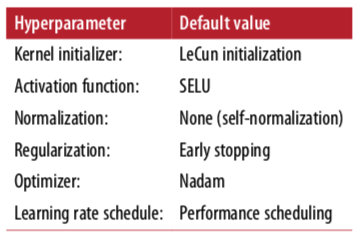
\includegraphics[scale=0.6]{img/config}
\caption{General configuration.}
\label{fig:config}
\end{figure}
Input features must be always standardised. Of course, you should also try to reuse parts of a pretrained neural network if you can find one that solves a similar problem, or use unsupervised pretraining if you have a lot of unlabeled data, or pretraining on an auxiliary task if you have a lot of labeled data for a similar task.

Some things might need adjustment:
\begin{itemize}
\item If your model self-normalizes:
	\begin{itemize}
		\item if it overfits the training set, then you should add alpha dropout (and always use early stopping as well). Do not use other regularization methods, or else they would break self-normalization.
	\end{itemize}
\item If your model cannot self-normalize (e.g., it is a recurrent net or it contains skip connections):
\begin{itemize}
\item You can try using ELU (or another activation function) instead of SELU, it may perform better. Make sure to change the initialization method accordingly (e.g., He initialisation for ELU or ReLU).
\item If it is a deep network, you should use Batch Normalization after every hidden layer. If it overfits the training set, you can also try using max-norm or L2 regularization.
\end{itemize}
\item If you need a sparse model, you can use L1 regularization (and optionally zero out the tiny weights after training). If you need an even sparser model, you can try using FTRL instead of Nadam optimization, along with l1 regularization. In any case, this will break self-normalization, so you will need to switch to BN if your model is deep.
\item If you need a low-latency model (one that performs lightning-fast predictions), you may need to use less layers, avoid Batch Normalization, and possibly replace the SELU activation function with the leaky ReLU. Having a sparse model will also help. You may also want to reduce the float precision from 32-bits to 16-bit (or even 8-bits).
\item If you are building a risk-sensitive application, or inference latency is not very important in your application, you can use MC Dropout to boost performance and get more reliable probability estimates, along with uncertainty estimates.
\end{itemize}
\printindex
